\documentclass[12pt, a4paper]{article}\usepackage[]{graphicx}\usepackage[]{xcolor}
% maxwidth is the original width if it is less than linewidth
% otherwise use linewidth (to make sure the graphics do not exceed the margin)
\makeatletter
\def\maxwidth{ %
  \ifdim\Gin@nat@width>\linewidth
    \linewidth
  \else
    \Gin@nat@width
  \fi
}
\makeatother

\definecolor{fgcolor}{rgb}{0.345, 0.345, 0.345}
\newcommand{\hlnum}[1]{\textcolor[rgb]{0.686,0.059,0.569}{#1}}%
\newcommand{\hlsng}[1]{\textcolor[rgb]{0.192,0.494,0.8}{#1}}%
\newcommand{\hlcom}[1]{\textcolor[rgb]{0.678,0.584,0.686}{\textit{#1}}}%
\newcommand{\hlopt}[1]{\textcolor[rgb]{0,0,0}{#1}}%
\newcommand{\hldef}[1]{\textcolor[rgb]{0.345,0.345,0.345}{#1}}%
\newcommand{\hlkwa}[1]{\textcolor[rgb]{0.161,0.373,0.58}{\textbf{#1}}}%
\newcommand{\hlkwb}[1]{\textcolor[rgb]{0.69,0.353,0.396}{#1}}%
\newcommand{\hlkwc}[1]{\textcolor[rgb]{0.333,0.667,0.333}{#1}}%
\newcommand{\hlkwd}[1]{\textcolor[rgb]{0.737,0.353,0.396}{\textbf{#1}}}%
\let\hlipl\hlkwb

\usepackage{framed}
\makeatletter
\newenvironment{kframe}{%
 \def\at@end@of@kframe{}%
 \ifinner\ifhmode%
  \def\at@end@of@kframe{\end{minipage}}%
  \begin{minipage}{\columnwidth}%
 \fi\fi%
 \def\FrameCommand##1{\hskip\@totalleftmargin \hskip-\fboxsep
 \colorbox{shadecolor}{##1}\hskip-\fboxsep
     % There is no \\@totalrightmargin, so:
     \hskip-\linewidth \hskip-\@totalleftmargin \hskip\columnwidth}%
 \MakeFramed {\advance\hsize-\width
   \@totalleftmargin\z@ \linewidth\hsize
   \@setminipage}}%
 {\par\unskip\endMakeFramed%
 \at@end@of@kframe}
\makeatother

\definecolor{shadecolor}{rgb}{.97, .97, .97}
\definecolor{messagecolor}{rgb}{0, 0, 0}
\definecolor{warningcolor}{rgb}{1, 0, 1}
\definecolor{errorcolor}{rgb}{1, 0, 0}
\newenvironment{knitrout}{}{} % an empty environment to be redefined in TeX

\usepackage{alltt}


%%%%%%%%%%%%%%%%%%%%%%%%%%%%%%%%%%%%%%%%%%%%%%%%%%%%%%%%%%%%%%%%
% additional LaTeX packages
% \usepackage[OT4]{polski}
\usepackage[utf8]{inputenc}
\usepackage[top=2.5cm, bottom=2.5cm, left=2cm, right=2cm]{geometry}
\usepackage{graphicx}
\usepackage{float}
\usepackage[colorlinks=true, linkcolor=blue]{hyperref}
\usepackage{anyfontsize}
\usepackage{bbm}
\usepackage{amsmath}
% \usepackage{Sweave}

%%%%%%%%%%%%%%%%%%%%%%%%%%%%%%%%%%%%%%%%%%%%%%%%%%%%%%%%%%%%%%%%

% global settings


\IfFileExists{upquote.sty}{\usepackage{upquote}}{}
\begin{document}
% \SweaveOpts{concordance=TRUE}

%%%%%%%%%%%%%%%%%%%%%%%%%%%%%%%%%%%%%%%%%%%%%%%%%%%%%%%%%%%%%%%%
\title{Advanced Applications of Statistical Packages\\
Report 1}
\author{Author 1, Author 2}
\maketitle
%\newpage

\tableofcontents 

%%%%%%%%%%%%%%%%%%%%%%%%%%%%%%%%%%%%%%%%%%%%%%%%%%%%%%%%%%%%%%%%
\newpage
%%%%%%%%%%%%%%%%%%%%%%%%%%%%%%%%%%%%%%%%%%%%%%%%%%%%%%%%%%%%%%%%

\section{Chunks}

We write R codes in chunks. Between $<<$ and $>\,>=$ we can put its name and local options. The global options can be given in the preamble. For example echo=TRUE shows (prints in the output PDF file) the results of the code, while echo=FALSE hides them. Another examples of chunk options can be found in the code of this file below.
You need to remember that each chunk must have different name. If the name is duplicated, the file may not compile, returning following error:

\texttt{processing file: FileName.rnw}

\texttt{Error in parse block(g[-1], g[1], params.src): duplicate label 'ChunkName'}

\texttt{Calls: knit process file split file lapply FUN parse block}

\texttt{Execution halted}


%%%%%%%%%%%%%%%%%%%%%%%%%%%%%%%%%%%%%%%%%%%%%%%%%%%%%%%%%%%%%%%%
%\newpage
\section{Simple data analysis}
\label{s:dataanalysis}
%%%%%%%%%%%%%%%%%%%%%%%%%%%%%%%%%%%%%%%%%%%%%%%%%%%%%%%%%%%%%%%%
We can import data set from a file or from URL using \texttt{read.csv} function.
\begin{knitrout}
\definecolor{shadecolor}{rgb}{0.969, 0.969, 0.969}\color{fgcolor}\begin{kframe}
\begin{alltt}
\hlcom{# 1. Importing data set from URL (CSV format)}
\hldef{url} \hlkwb{<-} \hlsng{"https://archive.ics.uci.edu/ml/machine-learning-databases/iris/iris.data"}
\hlcom{# Manually adding columns names}
\hldef{iris_data} \hlkwb{<-} \hlkwd{read.csv}\hldef{(url,} \hlkwc{header} \hldef{=} \hlnum{FALSE}\hldef{,}
                      \hlkwc{col.names} \hldef{=} \hlkwd{c}\hldef{(}\hlsng{"Sepal.Length"}\hldef{,} \hlsng{"Sepal.Width"}\hldef{,}
                                    \hlsng{"Petal.Length"}\hldef{,} \hlsng{"Petal.Width"}\hldef{,} \hlsng{"Species"}\hldef{))}
\end{alltt}
\end{kframe}
\end{knitrout}

A following code can be used to produce a simple table.
\begin{kframe}
\begin{alltt}
\hldef{summary_table} \hlkwb{<-} \hlkwd{summary}\hldef{(iris_data)}
\hlkwd{kable}\hldef{(summary_table,}
      \hlkwc{format} \hldef{=} \hlsng{"latex"}\hldef{,}
      \hlkwc{caption} \hldef{=} \hlsng{"Summary of Iris data set"}\hldef{)}
\end{alltt}
\end{kframe}\begin{table}

\caption{\label{tab:SummaryTable}Summary of Iris data set}
\centering
\begin{tabular}[t]{l|l|l|l|l|l}
\hline
  &  Sepal.Length &  Sepal.Width &  Petal.Length &  Petal.Width &   Species\\
\hline
 & Min.   :4.300 & Min.   :2.000 & Min.   :1.000 & Min.   :0.100 & Length:150\\
\hline
 & 1st Qu.:5.100 & 1st Qu.:2.800 & 1st Qu.:1.600 & 1st Qu.:0.300 & Class :character\\
\hline
 & Median :5.800 & Median :3.000 & Median :4.350 & Median :1.300 & Mode  :character\\
\hline
 & Mean   :5.843 & Mean   :3.054 & Mean   :3.759 & Mean   :1.199 & NA\\
\hline
 & 3rd Qu.:6.400 & 3rd Qu.:3.300 & 3rd Qu.:5.100 & 3rd Qu.:1.800 & NA\\
\hline
 & Max.   :7.900 & Max.   :4.400 & Max.   :6.900 & Max.   :2.500 & NA\\
\hline
\end{tabular}
\end{table}


Each table should have a caption above and it should be mentioned in the text.


\begin{figure}[H]
\begin{knitrout}
\definecolor{shadecolor}{rgb}{0.969, 0.969, 0.969}\color{fgcolor}\begin{kframe}
\begin{alltt}
\hlkwd{plot}\hldef{(iris_data}\hlopt{$}\hldef{Petal.Length, iris_data}\hlopt{$}\hldef{Petal.Width,}
     \hlkwc{col} \hldef{=} \hlkwd{as.factor}\hldef{(iris_data}\hlopt{$}\hldef{Species),} \hlcom{# Colouring by species}
     \hlkwc{pch} \hldef{=} \hlnum{19}\hldef{,}                           \hlcom{# point type - filled circle}
     \hlkwc{main} \hldef{=} \hlsng{"Plot of dependencies of petal length and width"}\hldef{,}
     \hlkwc{xlab} \hldef{=} \hlsng{"Petal length"}\hldef{,}
     \hlkwc{ylab} \hldef{=} \hlsng{"Petal width"}\hldef{)}

\hlcom{# list of points types:}
\hlcom{# https://www.sthda.com/english/wiki/r-plot-pch-symbols-the-different-point-shapes-available-in-r}

\hldef{pl_mean} \hlkwb{=} \hlkwd{round}\hldef{(}\hlkwd{mean}\hldef{(iris_data}\hlopt{$}\hldef{Petal.Length),} \hlnum{3}\hldef{)}

\hlcom{# Adding legend}
\hlkwd{legend}\hldef{(}\hlsng{"topleft"}\hldef{,} \hlkwc{legend} \hldef{=} \hlkwd{unique}\hldef{(iris_data}\hlopt{$}\hldef{Species),}
       \hlkwc{col} \hldef{=} \hlnum{1}\hlopt{:}\hlkwd{length}\hldef{(}\hlkwd{unique}\hldef{(iris_data}\hlopt{$}\hldef{Species)),} \hlkwc{pch} \hldef{=} \hlnum{19}\hldef{)}
\end{alltt}
\end{kframe}

{\centering 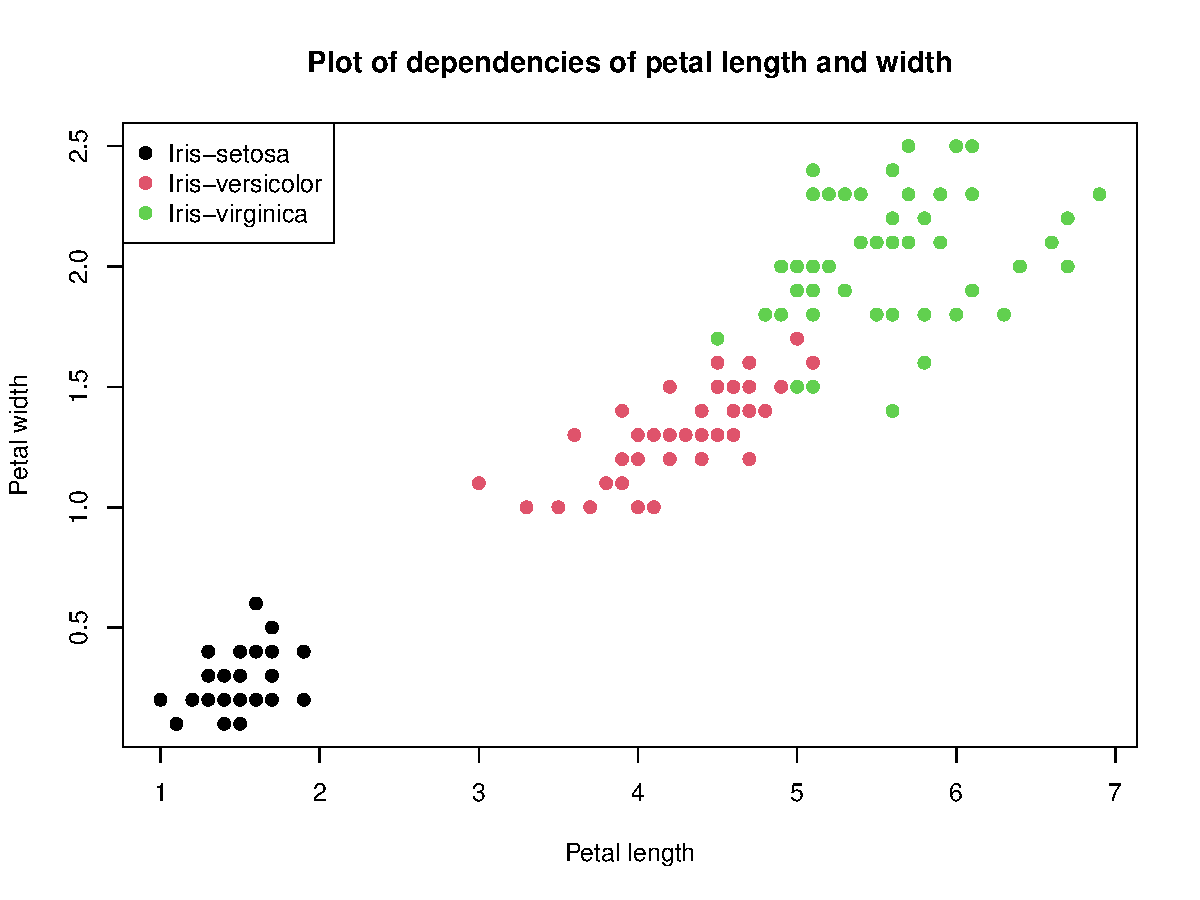
\includegraphics[width=\maxwidth]{figure/IrisPlot-1} 

}


\end{knitrout}
\caption{Plot of dependencies of petal length and width}
\label{fig:iris}
\end{figure}

Each figure should have a caption below. In the text there should be a reference to each figure. Simple plots for quick visualisations can be produced using native R functions \texttt{plot}, \texttt{curve}, \texttt{lines} or \texttt{boxplot}, but in a report it is required to use professional packages such as \texttt{ggplot2}. A function \texttt{ggplot} requires that its input is given as an object of type \textit{data.frame} (or \textit{tibble}). For a ggplot2 cheat sheet, see, for example, \url{https://miro.medium.com/v2/resize:fit:4800/format:webp/1*JXPvSBL-DxocIjdziCJkfw.jpeg}.

We can display the values of the variables computed in R chunks. For example, the average length of the petals in Iris data is 3.759. We can also performs simple computations inside \textit{Sexpr}, for example: 3.759.

%\newpage
R language has many functions which will be useful in this course, including:
\begin{itemize}
\item Basic statistics: \textit{mean}, \textit{median}, \textit{sum}, \textit{max} i \textit{min},
\item The \textit{which} function returns a vector containing indices where the argument is \texttt{TRUE}. It can be useful, for example, for finding the index of a vector's maximum, although you can also directly use the \textit{which.max} or which.min functions.
\item Finding the solution to an equation: \textit{uniroot} (Usage examples: [URL]).
\item Finding extrema of multivariable functions: \textit{optim} (Usage examples: [URL]).
\item Creating arithmetic sequences: \textit{seq}.
\item Creating lists (\textit{list}), vectors (\textit{c}), matrices (\textit{matrix}), and data frames (\textit{data.frame}).
\item Functions for changing data types: \textit{as.data.frame}, \textit{as.numeric}, \textit{as.character}, \textit{toString}.
\item Creating a table (or matrix or data frame) by binding rows (\textit{rbind}) or columns (\textit{cbind}) and assigning labels to rows (\textit{rownames}) and columns (\textit{colnames}).
\item Functions returning object sizes: \textit{length} (vector length), \textit{nrow} (number of rows), \textit{ncol} (number of columns), and \textit{dim} (number of rows and columns).
\end{itemize}

\section{Tips for creating reports}
Reports can be prepared using Sweave (rnw file) or Markdown (Rmd file). The report should be prepared in PDF format. The advantage of Sweave is its integration with \LaTeX, while the advantage of Markdown is its flexibility, thanks to which it can also be used to produce slide shows or HTML files. When creating your first report, you can use the attached template. It is also worth following the tips provided below.

\subsection{\LaTeX\ Notes}
\begin{itemize}
    \item 
When writing about variables in the text, e.g., sample $X$ or sample size $n$, use mathematical mode, i.e., write $X$ and not X.
    \item 
Functions (e.g., $\exp$ or $\min$) and operators (e.g., $\lim$) should be written using a backslash, i.e., do not write exp or lim, but \textbackslash exp or \textbackslash lim.
    \item 
It is better to write parentheses in the form \texttt{\textbackslash left(} ... \texttt{\textbackslash right)} rather than (...), because then their height adjusts to the size of the content.
\item 
English inserts (in case of reports written in different languages), function names, and package names should be written in italics.
\end{itemize}

\subsection{Writing code}
\begin{itemize}
    \item The report should include the code of functions in which calculations essential to solving the problem are performed. It is not necessary to include code used for generating plots, tables, etc. You also do not need to include auxiliary code used, for example, for transforming data frames with results.
    \item Reports should not contain information about errors and warnings. You can disable the insertion of such messages by placing \texttt{error=FALSE, warning=FALSE} in the chunk options or global options. Warnings usually concern library versions and can be ignored, whereas errors indicate that some part of our code failed to compile.
    \item Similarly, if a function "prints" unnecessary messages, they can be disabled by placing \texttt{message=FALSE} in the chunk options or global options. For some functions, you can also disable printing messages by calling the function with the argument \texttt{print=FALSE}.
    \item Unless specified that ready-made libraries can be used, solve the problems by writing functions yourself from scratch.
    \item Code placed in gray boxes (chunks) should not exceed the document margin. If it goes beyond the margin, you need to break the line. The limit is 79 characters (this may vary depending on font size or other factors).
    \item The code used for calculations does not have to be written in an optimal way, but it should not be written in an overly complex manner either.
    \item To minimize the risk of error, it is recommended that when performing complex calculations, you do not create dozens of separate variables for each set of considered parameters. It is recommended to keep each result in a single vector (or matrix). By creating a separate variable for each value placed in a table, you run the risk of making a mistake when entering variable names into the results matrix.
\end{itemize}

\subsection{Optimality of the code}
The fastest way for computing is using functions like \textit{colMeans}, \textit{colSums}, \textit{rowMeans} and \textit{rowSums} if possible. A bit slower are the apply-type functions, such as \textit{sapply}, \textit{lapply} etc. Using \textit{for} loops is the slowest option. Paralleling may increase the speed of the computations.
This is mostly important in case of simulation experiments or analysis of large data.

\subsection{Plots}
\begin{itemize}
\item 
Plots can be created in R using the \textit{ggplot2} package or using standard built-in functions in R (e.g., \textit{plot}, \textit{points}, \textit{curve}, and \textit{lines}). In the reports it is required to use \textit{ggplot2} or other professional package.
\item 
Figure captions are placed below the figures. A caption should not end with a period.
\item 
The caption should contain full information about the content of the plot; therefore, we should not write "CDF" or "Plot of CDF," but rather, e.g., "Plot of the cumulative distribution function of the exponential distribution with parameter $\lambda=4$". 
\item 
Every plot should contain a label (e.g., \textbackslash label\{fig:ExpCDF\}). Every figure should be referenced in the text (e.g., \textbackslash ref\{fig:ExpCDF\}). 
\item Both the horizontal and vertical axes should be labeled. Pay attention to whether the values on the vertical axis are correct, i.e. there should have range beyond minimum and maximum of the values presented on axis Y.
\item The plot should be large enough to read the information easily, but small enough not to take up the entire page. Sometimes it is more useful to create an illustration consisting of several small plots (an example can be found in the report template).
\end{itemize}

\subsection{Tables}
\begin{itemize}
\item Numbers in the table should be formatted in such a way that the results are legible and essential information can be read from it. For example, if the difference in the compared numbers is visible only at the fourth decimal place, we should display the results with 4 or 5 decimal places, rather than rounding to two decimal places.
\item If natural numbers are placed in a table (e.g., sample size or the number of observations having a certain characteristic), the column with such numbers should be formatted so that it does not display decimal places; thus, we do not write the number 10 as 10.0000.
\item 
Table captions are placed above the tables. A caption should not end with a period.
\item 
As with plots, the caption should contain full information about the content of the table. The table should contain a label and should be referenced in the text. 
\item Care should be taken not to incorrectly reference formulas, tables, and figures in the text ? this results in \textbf{??} appearing in the text. This may happen if we change the \textit{label} or if we place it in the wrong location.
\end{itemize}

\subsection{Inference}
\begin{itemize}
    \item If you see that you have obtained nonsensical results, do not include them in the report; instead, keep trying until you obtain sensible results. Usually, we know what the result should be based on intuition or classroom discussions.
    \item You should not include conclusions in the report that contradict the results presented in the table or on the plot.
    \item Solutions to problems involving simulations or data analysis should include conclusions that can be drawn from that analysis. 
    \item In the case of hypothesis testing, it is necessary to clearly state what the null and alternative hypotheses are. Furthermore, it is not enough to write the p-value; you must also write what decision should be made based on the obtained result.
\end{itemize}





\end{document}



